\subsubsection{Dimensionnement}

Comme pour le filtre passe-haut, on va utiliser le site internet \url{https://tools.analog.com/en/filterwizard/} pour dimensionner le filtre de garde. Nous avons cependant besoin d'introduire des informations concernant la "Passband region" et la "Stopband region", toutes les deux définies par une fréquence et un gain. Elles peuvent être déduites des conditions qui nous sont imposées sur le filtre. Pour rappel :

\begin{enumerate}
    \item[$\bullet$] Atténuation maximale des fréquences utiles : H1=0.99
    \item[$\bullet$] Atténuation minimale des fréquences repliées : H2=0.05
    \item[$\bullet$] Filtre d'ordre 2 (pour limiter le nombre d'étage de la chaîne analogique)
    \item[$\bullet$] Filtre de Butterworth (réponse la plus plate possible dans la bande passante)
\end{enumerate}

Sachant que la plus grande fréquence utile est $1100 \ Hz$ et que le gain d'un filtre de Butterworth d'ordre n a la forme suivante :

$$
||H(j\omega)|| = \sqrt{\frac{1}{1+\left(\frac{\omega}{\omega_c}\right)^{2n}}}
$$

On peut reformuler les contraintes :

\begin{align*}
\begin{cases}
||H(j \ 2 \pi1100 )||&=0.99 \\
||H(j \ 2 \pi f_{\text{repliement}})||&=0.05 \\
||H(j\omega)|| &= \sqrt{\frac{1}{1+\left(\frac{\omega}{\omega_c}\right)^{4}}}
\end{cases}
\end{align*}

On doit trouver la fréquence de coupure $\omega_c$ et la fréquence de repliement $f_{\text{repliement}}$ à partir de ces équations.

\begin{align*} 
||H(j2\pi 1100)|| &= \sqrt{\frac{1}{1+\left(\frac{2\pi 1100}{\omega_c}\right)^{4}}}\\
\iff ||H(j2\pi 1100)||^{2} \left(1+\left(\frac{2\pi 1100}{\omega_c}\right)^{4}\right) &= 1\\
\iff (\omega_c)^{4} &=\frac{1}{ \left(\frac{1}{||H(j2\pi 1100)||^{2}}-1\right) \frac{1}{(2\pi 1100)^{4}} }\\
\iff \omega_c&= 18309.51674 \ rad/s\\
\iff f_c &=  2914.050095 \ Hz
\end{align*}

\begin{align*} 
||H(j\omega_{\text{repliement}})|| &= \sqrt{\frac{1}{1+\left(\frac{\omega_{\text{repliement}}}{\omega_c}\right)^{4}}}\\
\iff ||H(j\omega_{\text{repliement}})||^{2} \left(1+\left(\frac{\omega_{\text{repliement}}}{\omega_c}\right)^{4}\right) &= 1\\
\iff (\omega_{\text{repliement}})^{4} &= \left(\frac{1}{||H(j\omega_{\text{repliement}})||^{2}}-1\right) {(\omega_c)^{4}} \\
\iff \omega_{\text{repliement}} &= 81831.42343 \ rad/s\\
\iff f_{\text{repliement}} &= 13023.87554 \ Hz
\end{align*}

En introduisant les valeurs suivantes pour le dimensionnement du filtre de garde :

\begin{align*}
\begin{cases}
\text{Passband region : }  f_c = 2914.050095 \ Hz & Gain=0dB \\
\text{Stopband region : }  f = 13023.87554 \ Hz  & Gain=-26.02dB
\end{cases}
\end{align*}

On obtient le filtre de la figure \ref{fig:filtregarde}. Les détails des données introduites sur le site pour le filtre sont disponibles dans l'Annexe \ref{Lowpassfilterannexe}.

\begin{figure}[H]
    \centering
    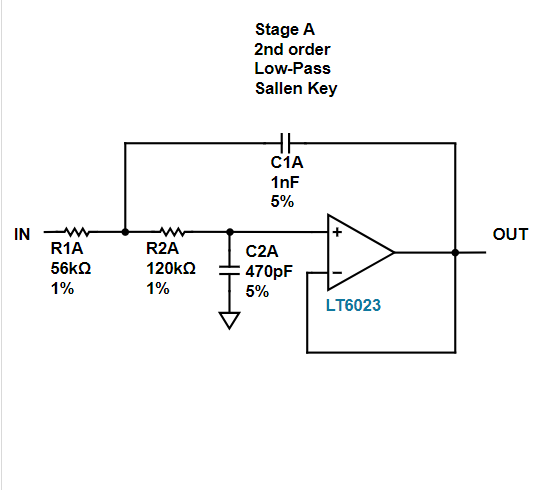
\includegraphics[width=0.5\textwidth]{Pictures/lowpass2.png}
    \caption{Filtre de Butterworth d'ordre 2}
    \label{fig:filtregarde}
\end{figure}

Le dimensionnement du filtre de garde s'arrête ici, on peut directement ajouter cet étage en cascade avec le premier et passer à la validation du bloc \textbf{Filtre de garde}.

\subsubsection{Validation du bloc}

Pour valider ce bloque indépendamment du bloc \textbf{Amplification}, on peut générer un signal sinusoïdal avec le Picoscope et observer l'atténuation du signal de sortie avec l'augmentation de la fréquence.
